\section{Tools used}
\subsection{Buildroot}
Buildroot is a set of Makefiles and patches that simplifies and automates the process of building a complete and bootable Linux environment for an embedded system, while using cross-compilation to allow building for multiple target platforms on a single Linux-based development system. Buildroot can automatically build the required cross-compilation toolchain, create a root file system, compile a Linux kernel image, and generate a boot loader for the targeted embedded system, or it can perform any independent combination of these steps. For example, an already installed cross-compilation toolchain can be used independently, while Buildroot only creates the root file system. \\
Buildroot is primarily intended to be used with small or embedded systems based on various computer architectures and instruction set architectures (ISAs), including x86, ARM, MIPS and PowerPC. Numerous architectures and their variants are supported; Buildroot also comes with default configurations for several off-the-shelf available embedded boards, such as Cubieboard, Raspberry Pi and SheevaPlug. Several third-party projects and products use Buildroot as the basis for their build systems, including the OpenWrt project that creates an embedded operating system, and firmware for the customer-premises equipment (CPE) used by the Google Fiber broadband service.\\
Multiple C standard libraries are supported as part of the toolchain, including the GNU C Library, uClibc and musl, as well as the C standard libraries that belong to various preconfigured development environments, such as those provided by Linaro. Buildroot's build configuration system internally uses Kconfig, which provides features such as a menu-driven interface, handling of dependencies, and contextual help; Kconfig is also used by the Linux kernel for its source-level configuration. Buildroot is organized around numerous automatically downloaded packages, which contain the source code of various userspace applications, system utilities, and libraries. Root file system images, which are the final results, may be built using various file systems, including cramfs, JFFS2, romfs, SquashFS and UBIFS.\\
Buildroot is free and open-source software, maintained by Peter Korsgaard and licensed under version 2 or later of the GNU General Public License (GPL). The project started in 2001, with initial intentions to serve as a testbed for uClibc. New releases are made available every three months.
\begin{figure}[ht]
	\centering
	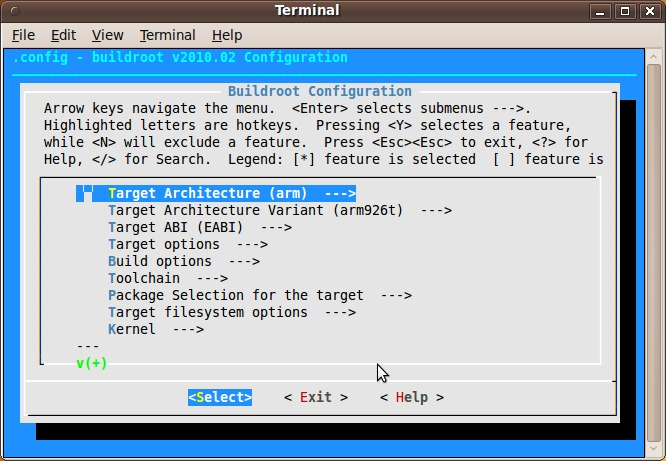
\includegraphics[width=3.5in, height=3in]{images/buildroot.png}
	\caption{Buildroot}
\end{figure}
\subsection{Cscope}
While hacking around the Linux source code it becomes very difficult to keep track of the program flow or the variable structures in your head. There isn’t any IDE to help out in source code browsing either. In such situation a tool is necessary that browses source code and is based on the terminal. This is where cscope comes into picture.\\
cscope is a programming tool which works in console mode, text-based interface, that allows computer programmers or software developers to search source code of the programming language C, with some support for C++ and Java. It is often used on very large projects to find source code, functions, declarations, definitions and regular expressions given a text string. cscope is free and released under a BSD license. The original developer of cscope is \textbf{Joe Steffen}.\\
The history of the tool goes back to the days of the PDP-11, but it is still used by developers who are accustomed to using the vi or Vim editor or other text-based editors, instead of editors based on graphical user interfaces (GUI)s. The functions in cscope are available to varying degrees in modern graphical source editors.
cscope is used in two phases. First a developer builds the cscope database. The developer can often use find or other Unix tools to get the list of filenames needed to index into a file called cscope.files. The developer then builds a database using the command cscope -b -q -k. The k flag is intended to build a database for an operating system or C library source code. It will not look in /usr/include. Second, the developer can now search those files using the command cscope -d. Often an index must be rebuilt whenever changes are made to files.\\
In software development it is often very useful to be able to find the callers of a function because this is the way to understand how code works and what other parts of the program expect from a function. cscope can find the callers and callees of functions, but it is not a compiler and it does that by searching the text for keywords. This has the disadvantages that macros and duplicate symbol names can generate an unclear graph. There are other programs that can extract this information by parsing the source code or looking at the generated object files.
cscope was created to search content within C files, but it can also be used (with some limits) for C++ and Java files.
\begin{figure}[ht]
	\centering
	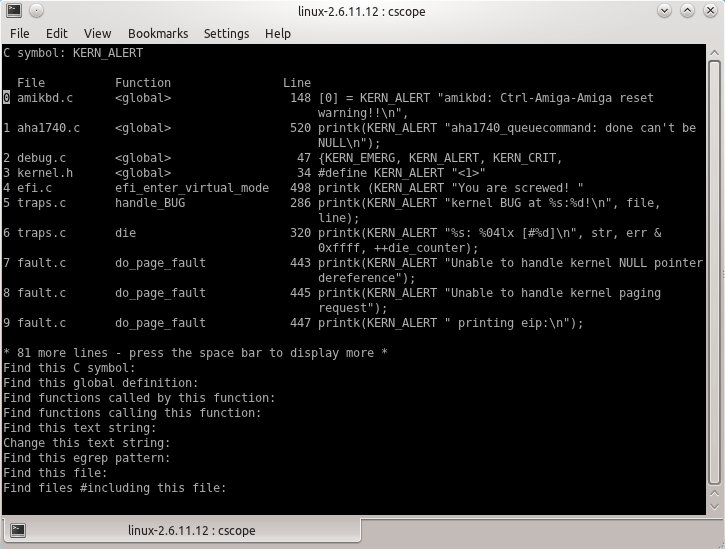
\includegraphics[scale=0.5]{images/cscope.png}
	\caption{Source Browsing through Cscope}
\end{figure}
